%header and footer for separate chapter files

\ifx\whole\undefined
\documentclass[12pt, leqno]{book}
\usepackage{graphicx}
\input style-for-curves.sty
\usepackage{hyperref}
\usepackage{showkeys} %This shows the labels.
%\usepackage{SLAG,msribib,local}
%\usepackage{amsmath,amscd,amsthm,amssymb,amsxtra,latexsym,epsfig,epic,graphics}
%\usepackage[matrix,arrow,curve]{xy}
%\usepackage{graphicx}
%\usepackage{diagrams}
%
%%\usepackage{amsrefs}
%%%%%%%%%%%%%%%%%%%%%%%%%%%%%%%%%%%%%%%%%%
%%\textwidth16cm
%%\textheight20cm
%%\topmargin-2cm
%\oddsidemargin.8cm
%\evensidemargin1cm
%
%%%%%%Definitions
%\input preamble.tex
%\input style-for-curves.sty
%\def\TU{{\bf U}}
%\def\AA{{\mathbb A}}
%\def\BB{{\mathbb B}}
%\def\CC{{\mathbb C}}
%\def\QQ{{\mathbb Q}}
%\def\RR{{\mathbb R}}
%\def\facet{{\bf facet}}
%\def\image{{\rm image}}
%\def\cE{{\cal E}}
%\def\cF{{\cal F}}
%\def\cG{{\cal G}}
%\def\cH{{\cal H}}
%\def\cHom{{{\cal H}om}}
%\def\h{{\rm h}}
% \def\bs{{Boij-S\"oderberg{} }}
%
%\makeatletter
%\def\Ddots{\mathinner{\mkern1mu\raise\p@
%\vbox{\kern7\p@\hbox{.}}\mkern2mu
%\raise4\p@\hbox{.}\mkern2mu\raise7\p@\hbox{.}\mkern1mu}}
%\makeatother

%%
%\pagestyle{myheadings}

%\input style-for-curves.tex
%\documentclass{cambridge7A}
%\usepackage{hatcher_revised} 
%\usepackage{3264}
   
\errorcontextlines=1000
%\usepackage{makeidx}
\let\see\relax
\usepackage{makeidx}
\makeindex
% \index{word} in the doc; \index{variety!algebraic} gives variety, algebraic
% PUT a % after each \index{***}

\overfullrule=5pt
\catcode`\@\active
\def@{\mskip1.5mu} %produce a small space in math with an @

\title{Personalities of Curves}
\author{\copyright David Eisenbud and Joe Harris}
%%\includeonly{%
%0-intro,01-ChowRingDogma,02-FirstExamples,03-Grassmannians,04-GeneralGrassmannians
%,05-VectorBundlesAndChernClasses,06-LinesOnHypersurfaces,07-SingularElementsOfLinearSeries,
%08-ParameterSpaces,
%bib
%}

\date{\today}
%%\date{}
%\title{Curves}
%%{\normalsize ***Preliminary Version***}} 
%\author{David Eisenbud and Joe Harris }
%
%\begin{document}

\begin{document}
\maketitle

\pagenumbering{roman}
\setcounter{page}{5}
%\begin{5}
%\end{5}
\pagenumbering{arabic}
\tableofcontents
\fi


\chapter{Hyperelliptic curves and curves of genus 2 and 3}\label{genus 2 and 3 chapter}

\section{Hyperelliptic Curves}
 
 
In the world of curves, hyperelliptic curves are outliers: they behave differently from other curves, and the techniques used to analyze them are different from the techniques used for more general curves. Many theorems about curves contain the hypothesis ``non-hyperelliptic," with the corresponding result for hyperelliptic curves arrived at directly by ad hoc methods. Because the methods of this section will not be used in other cases, it could be skipped in first reading
 
%There will be a further discussion of hyperelliptic curves in Chapter~\ref{ScrollsChapter}, focussing on the algebra and geometry of their projective embeddings; the analysis here will cover most of the questions we'll be asking about curves in general in the next four chapters. 
  
 \subsection{The equation of a hyperelliptic curve}
 
By definition, a hyperelliptic curve $C$ is one admitting a degree two map $\pi : C \to \PP^1$. Because the degree is only 2, each point in $\PP^1$ has either two distinct preimages, or one point of simple ramification. There can be no higher ramification, so at all but finitely many points $p \in C$ the map $\pi$ is a local isomorphism (``local" here in the complex analytic/classical or \'etale topology, not the Zariski topology!); at any other point $p \in C$, the map is given in terms of local analytic coordinates on $C$ and $\PP^1$ simply by $z \mapsto z^2$. In particular, both the ramification divisor and the branch divisor (as defined in Chapter~\ref{linear systems chapter}) are reduced. Thus by the Riemann-Hurwitz formula there are exactly $2g+2$ branch points $q_1,\dots,q_{2g+2} \in \PP^1$. These points determine the curve:
  
 
\begin{theorem}\label{hyperelliptic existence}
There is a unique smooth projective hyperelliptic curve $C$ expressible as a 2-sheeted cover of $\PP^1$ branched over any set of $2g+2$ distinct points.
\end{theorem}

\begin{proof} 
We can easily construct such a curve, postponing for a moment the uniqueness:
If the coordinate of the point $p_i \in \PP^1$ is $\lambda_i$, it is the smooth projective model of the affine curve 
  $$
C^\circ = \big\{ (x,y) \in \AA^2 \; \mid \; y^2 = \prod_{i=1}^{2g+2} (x - \lambda_i) \big\}.
$$ 
Note that we're choosing a coordinate $x$ on $\PP^1$ with the point $x = \infty$ at infinity not among the $q_i$, so that the pre-image of $\infty \in \PP^1$ is two points $r, s \in C$. Concretely, we see that as $x \to \infty$, the ratio $y^2/x^{2g+2} \to 1$, so that 
$$
\lim_{x \to \infty} \; \frac{y}{x^{g+1}} \; = \; \pm 1;
$$
  the two possible values of this limit correspond to the two points $r,s \in C$.
  
  It's worth pointing out that $C$ is \emph{not} simply the closure of the affine curve $C^\circ \subset \AA^2$ in either $\PP^2$ or $\PP^1 \times \PP^1$: as you can see from a direct examination of the equation, each of these closures will be singular at the (unique) point at infinity.
  
   The remainder of the proof of Theorem~\ref{hyperelliptic existence} will be a special case of the  description of branched covers of curves in general given in Section~\ref{branched covers} below.
   
 \begin{exercise}
  In the case $g=1$, show that the closure $\overline{C^\circ}$ of $C^\circ \subset \AA^2$ in either $\PP^2$ or $\PP^1 \times \PP^1$ consists of the union of $C^\circ$ with one additional point, with that point a tacnode of $\overline{C^\circ}$ in either case.
  \end{exercise}
  
It is also possible to give a projective model of the hyperelliptic curve $C$ with given branch divisor: if we divide the points $q_1,\dots,q_{2g+2} \in \PP^1$ into two sets of $g+1$---say, for example, $q_1,\dots,q_{g+1}$ and $q_{g+2}, \dots, q_{2g+2}$---then $C$ is the closure in $\PP^1 \times \PP^1$ of the  locus
  $$
  \big\{ (x,y) \in \AA^2 \; \mid \; y^2\prod_{i=1}^{g+1} (x - \lambda_i) = \prod_{i=g+2}^{2g+2} (x - \lambda_i) \big\};
  $$
  in projective coordinates, this is
   $$
  C \; = \; \big\{ (X,Y) \in \PP^1 \times \PP^1 \; \mid \; Y_1^2\prod_{i=1}^{g+1} (X_1 - \lambda_iX_0) = Y_0^2\prod_{i=g+2}^{2g+2} (X_1 - \lambda_iX_0) \big\}.
  $$
  (No local analysis is needed to see that $C \subset \PP^1 \times \PP^1$ is smooth: it is a curve of bidegree $(2,g+1)$ in $\PP^1 \times \PP^1$, and the formula for the genus of a curve in $\PP^1 \times \PP^1$ derived in Section~\ref{rational quartics section} tells us that such a curve has arithmetic genus $g$.)
  
  Finally, note that the map $\iota : C \to C$ that exchanges the two points in each reduced fiber of the map $C \to \PP^1$ and fixes the ramification points is visibly algebraic (for example, in terms of the last representation of $C$, it is given simply by $([X_0,X_1], [Y_0,Y_1]) \mapsto  ([X_0,X_1], [Y_0,-Y_1]) $). The map $\iota$ is called the \emph{hyperelliptic involution} on $C$.



%  \
%  
%  \
%  
%  \
%  
%  \
% 
% We start by establishing some basic facts about hyperelliptic curves. Many of these follow from general theorems like Riemann-Roch; but since they can be established by direct examination we will carry that out here.
%
%Suppose $C$ is a smooth, projective hyperelliptic curve of genus $g \geq 2$. By definition, $C$ admits a degree 2 map $\pi : C \to \PP^1$; and as we've observed (\ref{**}) this map is unique.
%
%By Riemann-Hurwitz, \fix{attibution?} the map $\pi : C \to \PP^1$ will have $2g+2$ distinct simple branch points, say $\lambda_1,\dots,\lambda_{2g-2} \in \PP^1$. An open subsect $C^\circ$ of $C$ can then be realized as the smooth projective completion of the affine curve given as
%$$
%C^\circ = \big\{ (x,y) \in \AA^2 \; \mid \; y^2 = \prod_{i=1}^{2g+2} (x - \lambda_i) \big\}.
%$$ 
%\fix{if two of the $\lambda_i$ coinncide, then the curve develops a singular point. Much of what we will do carries over to the singular case.} \fix{say the smooth model has 2 points at $\infty$.} Note that if we simply take the closure of this locus in $\PP^2$, the resulting curve will be highly singular at the point $[1,0,0]$, as can be seen either  directly by making an appropriate change of variables, or by invoking the genus formula for plane curves: if the closure were smooth, it would have genus $\binom{2g+1}{2}$. We can, however, complete the curve simply in $\PP^1 \times \PP^1$, for example by setting \fix{this is a rabbit from a hat. Consider either saying that by the previous section, if there's an emb in P3 then its on P1 x P1 as a divisor of type
%2,g+1; and then "finding" this embedding as below; or moving this page to the early place where hyperelliptic curves are first mentioned.}
%$$
%y' = \frac{y}{\prod_{i=1}^{g+1} (x - \lambda_i)};
%$$
%we can then write the equation of a still smaller open subset of $C$ as
%$$
%{y'}^2 \cdot \prod_{i=1}^{g+1} (x - \lambda_i) \; = \; \prod_{i=g+2}^{2g+2} (x - \lambda_i).
%$$
%If we now take the closure of this locus in $\PP^1 \times \PP^1$, we get a curve of type $(2,g+1)$ on $\PP^1 \times \PP^1$; this curve is smooth, as can be seen again either directly in coordinates or by invoking the genus formula for curves on $\PP^1 \times \PP^1$. In other words,
%$$
%C \; = \; V\Big(Y_0^2\cdot \prod_{i=1}^{g+1} (X_1 - \lambda_iX_0) - Y_1^2 \cdot \prod_{i=g+2}^{2g+2} (X_1 - \lambda_iX_0) \Big)
%$$

  
  \subsection{Differentials on a hyperelliptic curve}

We can give a very concrete description of the differentials, and thus the canonical linear series, on a hyperelliptic curve $C$ by working with the affine model $C^\circ = V(f) \subset \AA^2$, where
$$
f(x,y) = y^2 - \prod_{i=1}^{2g+2} (x - \lambda_i).
$$
We will again denote the two points at infinity---that is, the two points of $C \setminus C^\circ$ by $r$ and $s$; for convenience, we'll denote the divisor $r+s$ by $D$.

To start, consider the simple differential $dx$ on $C$. (Technically, we should write this as $\pi^*dx$, since we mean the pullback to $C$ of the differential $dx$ on $\PP^1$, but for simplicity of notation we'll suppress the $\pi^*$.)  The function $x$ is regular on $C^\circ$, and is a local parameter over points other than the $\lambda_i$; from the local description of the map $\pi$, we see that $dx$ is regular on $C^\circ$  with simple zeros at the ramification points $q_i = (\lambda_i, 0)$. But it does not extend to a regular differential on all of $C$: it will have double poles at $r$ and $s$.  This can be seen directly: the differential $dx$ extends to a rational differential on $\PP^1$, and in terms of the local coordinate $w = 1/x$ around the point $x = \infty$ on $\PP^1$, we have
$$
dx = d\left(\frac{1}{w}\right) = \frac{-dw}{w^2}
$$
so $dx$ has a double pole at the point at $\infty$; since the map $\pi$ is a local isomorphism near $r$ and $s$ the pullback of $dx$ to $C$ likewise has double poles at the points $r$ and $s$.


We could also see that $dx$ must have poles by degree considerations: as we said, $dx$ has $2g+2$ zeros and no poles in $C^\circ$, while the degree of $K_C$ is $2g-2$, meaning that there must be  a total of four poles at the points $r$ and $s$. In any event, we have an expression for the canonical divisor class on $C$: denoting by $R = q_1 + \dots + q_{2g+2}$ the sum of the ramifications points of $\pi$, we have
$$
K_C \sim (dx) \sim R - 2D;
$$
this is a case of the Riemann-Hurwitz of Chapter~\ref{linear systems chapter}.

So, given that $dx$ has poles at $r$ and $s$, how do we find regular differentials on $C$? One thing to do would be simply to divide by $x^2$ (or any quadratic polynomial in $x$) to kill the poles. But that just introduces new poles in the finite part $C^\circ$ of $C$. Instead, we want to multiply $dx$ by a rational function with zeros at $p$ and $q$, but \emph{whose poles occur only at the points where $dx$ has zeroes}---that is, the points $q_i$.  A natural choice is simply the reciprocal of the partial derivative $f_y = \partial f/ \partial y = 2y$, which vanishes exactly at the points $q_i$, and has correspondingly a pole of order $g+1$ at each of the points $r$ and $s$ (reason: the involution $y\to -y$ fixes $C^\circ$ and $x$, and exchanges the points $r$ and $s$). In other words, as long as $g \geq 1$, the differential
$$
\omega = \frac{dx}{f_y}
$$
is regular, with divisor
$$
(\omega) = (g-1)r + (g-1)s = (g-1)D.
$$
The remaining regular differentials on $C$ are now easy to find: Since $x$ has only a simple pole
at the two points at infinity we can  multiply $\omega$ by any $x^k$ with $k = 0, 1, \dots, g-1$. Since this gives us $g$ independent differentials, we see that the differentials
$$
\omega, x\omega, \dots, x^{g-1}\omega
$$
  form a basis for $H^0(K_C)$.

\subsection{The canonical map of a hyperelliptic curve}\label{hyperelliptic special}

Given that a basis for $H^0(K_C)$ is given by 
$$
H^0(K_C) = \langle \omega, x\omega,\dots,x^{g-1}\omega \rangle,
$$
we see that the canonical map $\phi : C \to \PP^{g-1}$ is given by $[1,x,\dots,x^{g-1}]$. In other words, the canonical map $\phi$ is simply the composition of the map $\pi : C \to \PP^1$ with the Veronese embedding $\PP^1 \hookrightarrow \PP^{g-1}$ of $\PP^1$ into $\PP^{g-1}$ as a rational normal curve of degree $g-1$.

Note that as a consequence of this fact, we see that \emph{a hyperelliptic curve $C$ has a \emph{unique} linear series $g^1_2$ of degree 2 and dimension 1}: the $g^1_2$ is characterized as the complete linear system $|D|$, where $D$ is the sum of any two points mapping to the same point under the canonical map. Equivalently, we see that $C$ admits  a unique map of degree 2 to $\PP^1$. 

Finally, we can give an explicit description of special linear series on a hyperelliptic curve: if $D = \sum p_i$ is any effective divisor on $C$, we can pair up points $p_i$ that are conjugate under the involution $\iota$ exchanging sheets of the degree 2 map $C \to \PP^1$; each conjugate pair is a divisor of the unique $g^1_2$ on $C$, and so we can write
$$
D \sim r\cdot g^1_2 + q_1 + \dots + q_{d-2r},
$$
where no two of the points $q_i$ are conjugate under $\iota$. Now the geometric form of the Riemann-Roch formula tells us that the dimension $r(D)$ of the complete linear series $|D|$ is exactly $r$, so that in fact 
$$
|D| = |r\cdot g^1_2| + q_1 + \dots + q_{d-2r};
$$
that is, the points $q_i$ are base points of the linear series $|D|$.

One key observation is that, according to this analysis, \emph{no special linear series on a hyperelliptic curve can be very ample}; the map associated to any special series factors through the degree 2 map $C \to \PP^1$. This is in marked contrast to the case of non-hyperelliptic curves of genus $g \geq 3$, for which the embeddings of minimal degree in projective space are given by special linear series. 

   \subsection{Interlude: branched covers with specified branch divisor}\label{branched covers}
   
   We will describe here the classification of branched covers $\pi : C \to B$ of a given curve $B$ with specified branch points. To give ourselves a concrete goal, we will address the question: given a curve $B$ and a collection $\Delta = \{p_1,\dots,p_b\} \subset B$ of points in $B$, how many branched covers $\pi : C \to B$ of degree $d$ are there with specified branching over each of the points $p_i$, up to isomorphism over $B$? Our analysis will consist of two steps: first, we will reduce the problem to the classification of topological covering spaces of the complement $U = B \setminus \Delta$; we will then use our knowledge of the fundamental group of $U$ to enumerate such covering spaces.
   
   For the first step, we claim that \emph{given any topological covering space $\pi^\circ : V \to U$, the 2-manifold $V$ may be given the structure of a Riemann surface in a unique way so that the map $\pi^\circ$ is holomorphic; and $V$ may be compactified to a compact Riemann surface $C$ such that the map $\pi^\circ$ extends to a holomorphic map $\pi : C \to B$, again in a unique way.} The first statement---that $V$ inherits the structure of a complex manifold from $U$---is clear: if $D \subset U$ is any simply connected coordinate chart, the preimage $({\pi^\circ})^{-1}(D)$ will be a disjoint union of $d$ copies of $D$; these will serve as coordinate charts on $V$. 
   
   As for the compactification, we observe that if $D^* = \{ z \in \CC \mid 0 < |z| < 1 \}$ is a punctured disc, then \emph{any connected finite covering space of $D^*$, with the inherited complex structure, is again biholomorphic to a punctured disc}; thus if $D_i$ is a small neighborhood of the point $p_i \in B$ biholomorphic to a disc, then the preimage of the punctured disc $D_i^* := D_i \cap U$ in $V$ is a disjoint union of punctured discs; $V$ can then be compactified to a compact Riemann surface by completing each one to a full disc.
   
%   So: let's suppose that $q_1, \dots ,q_b \in \PP^1$ are any $b$ given points; we want to describe covers $C \to \PP^1$ of degree $d$ simply branched over the points $q_i$ (so that $b = 2d + 2g - 2$, where $g$ is the genus of $C$). To begin with, let $\Delta = \{q_1,\dots,q_b\}$ be the set of branch points, and choose a base point $p \in \PP^1$ not in $\Delta$, and let $\gamma_1, \dots, \gamma_b$ be simple arcs joining $p$ to the points $q_i$, disjoint except for their initial point $p$.
%   
%   One point to establish right away is this: if $\pi : C \to B$ is a branched cover, branched over $\Delta = \{q_1,\dots,q_b\} \subset B$, let $U = B \setminus \Delta$ be the complement of the branch locus and $V = \pi^{-1}(U) \subset C$. The restriction $\pi^\circ = \pi |_{V} : V \to U$ is then a topological covering space in the classical topology, and we claim that \emph{we have a bijection between connected, degree $d$ covering spaces of $U$ and smooth, projective curves $C$ with a map $\pi : C \to B$ of degree $d$}---in other words, any topological covering space $V \to U$ of $U$ can be compactified and given the structure of a Riemann surface in such a way that the map $V \to U$ extends to a holomorphic map $C \to B$, and this extension is unique.
%   
%   The proof of this assertion is straightforward. Let $V \to U$ be a covering space. If $D_\alpha$ is a small ball around the branch point $q_\alpha$, let $D^*_\alpha = D_\alpha \cap U = D_\alpha \setminus \{q_\alpha\}$ be the corresponding punctured disc. The preimage of $D^*_\alpha$ in $V$ is then a covering space of the punctured disc, and so must be a disjoint union of punctured discs. We can then complete each of these punctured discs to a disc by adding one point, which maps to $q_alpha$. The resulting compact surface $C$ can then be given the structure of a Riemann surface such that the extended map $\pi : C \to B$ is holomorphic.
   
   Given the bijection between connected, degree $d$ covering spaces of $U$ and smooth, projective curves $C$ with a map $\pi : C \to B$ of degree $d$, the problem becomes one of classifying covering spaces of $U$. To carry this out, we'll deal first with the case where  $B = \PP^1$ and $\pi : C \to \PP^1$ is simply branched; we'll indicate how the more general problem goes in Exercises~\ref{} and \ref{}.
   
   We start by drawing the classical picture. Choose a base point $p_0 \in U$, and draw simple, non-intersecting arcs $\gamma_i$ joining $p_0$ to $p_i$ in $U$. If $\Sigma$ is the complement of the union of these arcs in the sphere, then the preimage of $\Sigma$ in $V$ will be the disjoint union of $d$ copies of $\Sigma$, called the \emph{sheets} of the cover; label these $\Sigma_1,\dots,\Sigma_d$
   
%   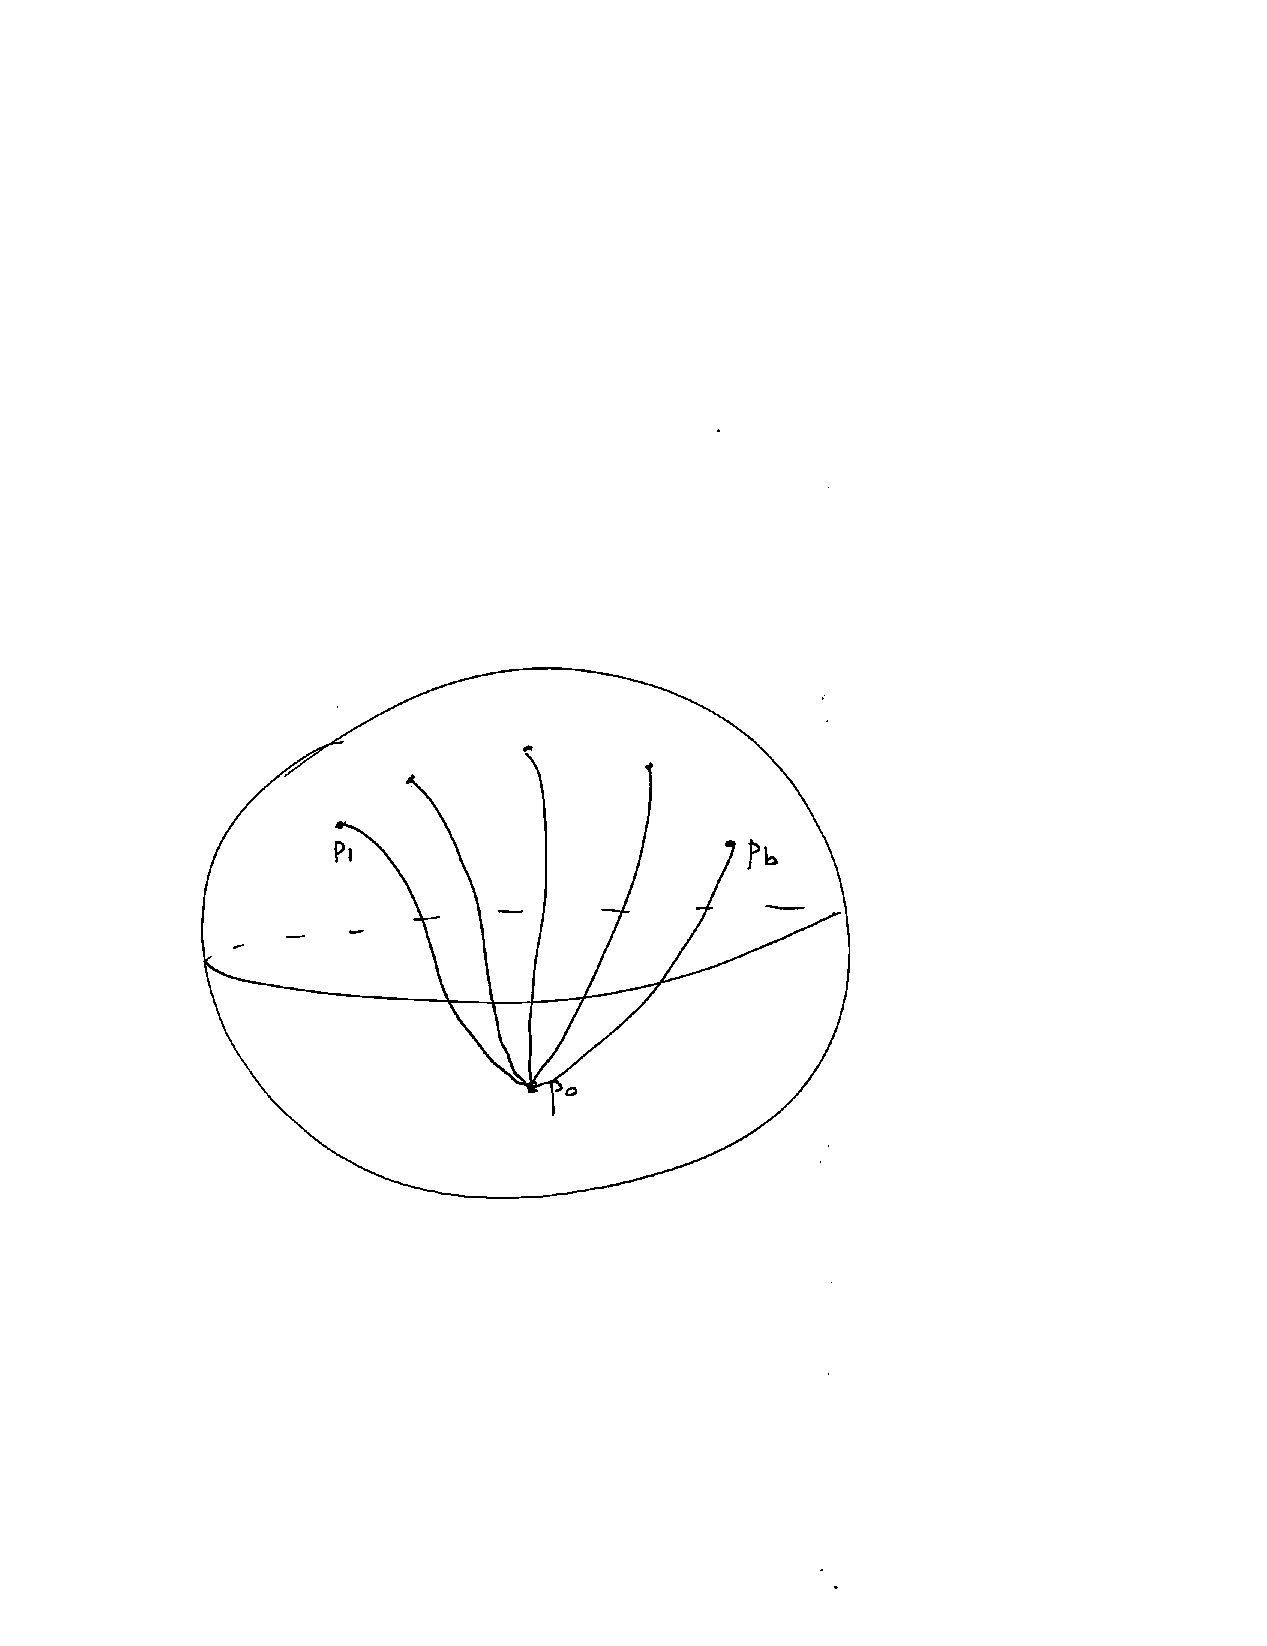
\includepdf{pic4.1}
   
   Now, covering spaces $V \to U$ of $U$ are classified by their \emph{monodromy}, which is the map
   $$
   \pi_1(U, p_0) \to S_d
   $$
   associating to each loop $\beta$ in $U$ the permutation of the points of $\pi^{-1}(p_0)$ given by sending a point $q \in \pi^{-1}(p_0)$ to the endpoint of the unique lift of $\beta$ starting at $q$. Now, let $\beta_i$ be a loop starting at $p_0$, going out along the arc $\gamma_i$ until just short of $p_i$, going once around $p_i$ and then going back to $p_0$ along the same path $\gamma_i$, as drawn in the Figure, and let $\tau_i$ be the corresponding permutation of $\{1,2,\dots,d\}$. The loops $\beta_i$  generate the fundamental group $\pi_1(U, p_0)$, with the one relation that the product $\beta_1\cdot \dots \cdot \beta_b = Id$ is the identity; the permutations $\tau_1,\dots,\tau_b$ thus determine the covering space $V$.
   
%   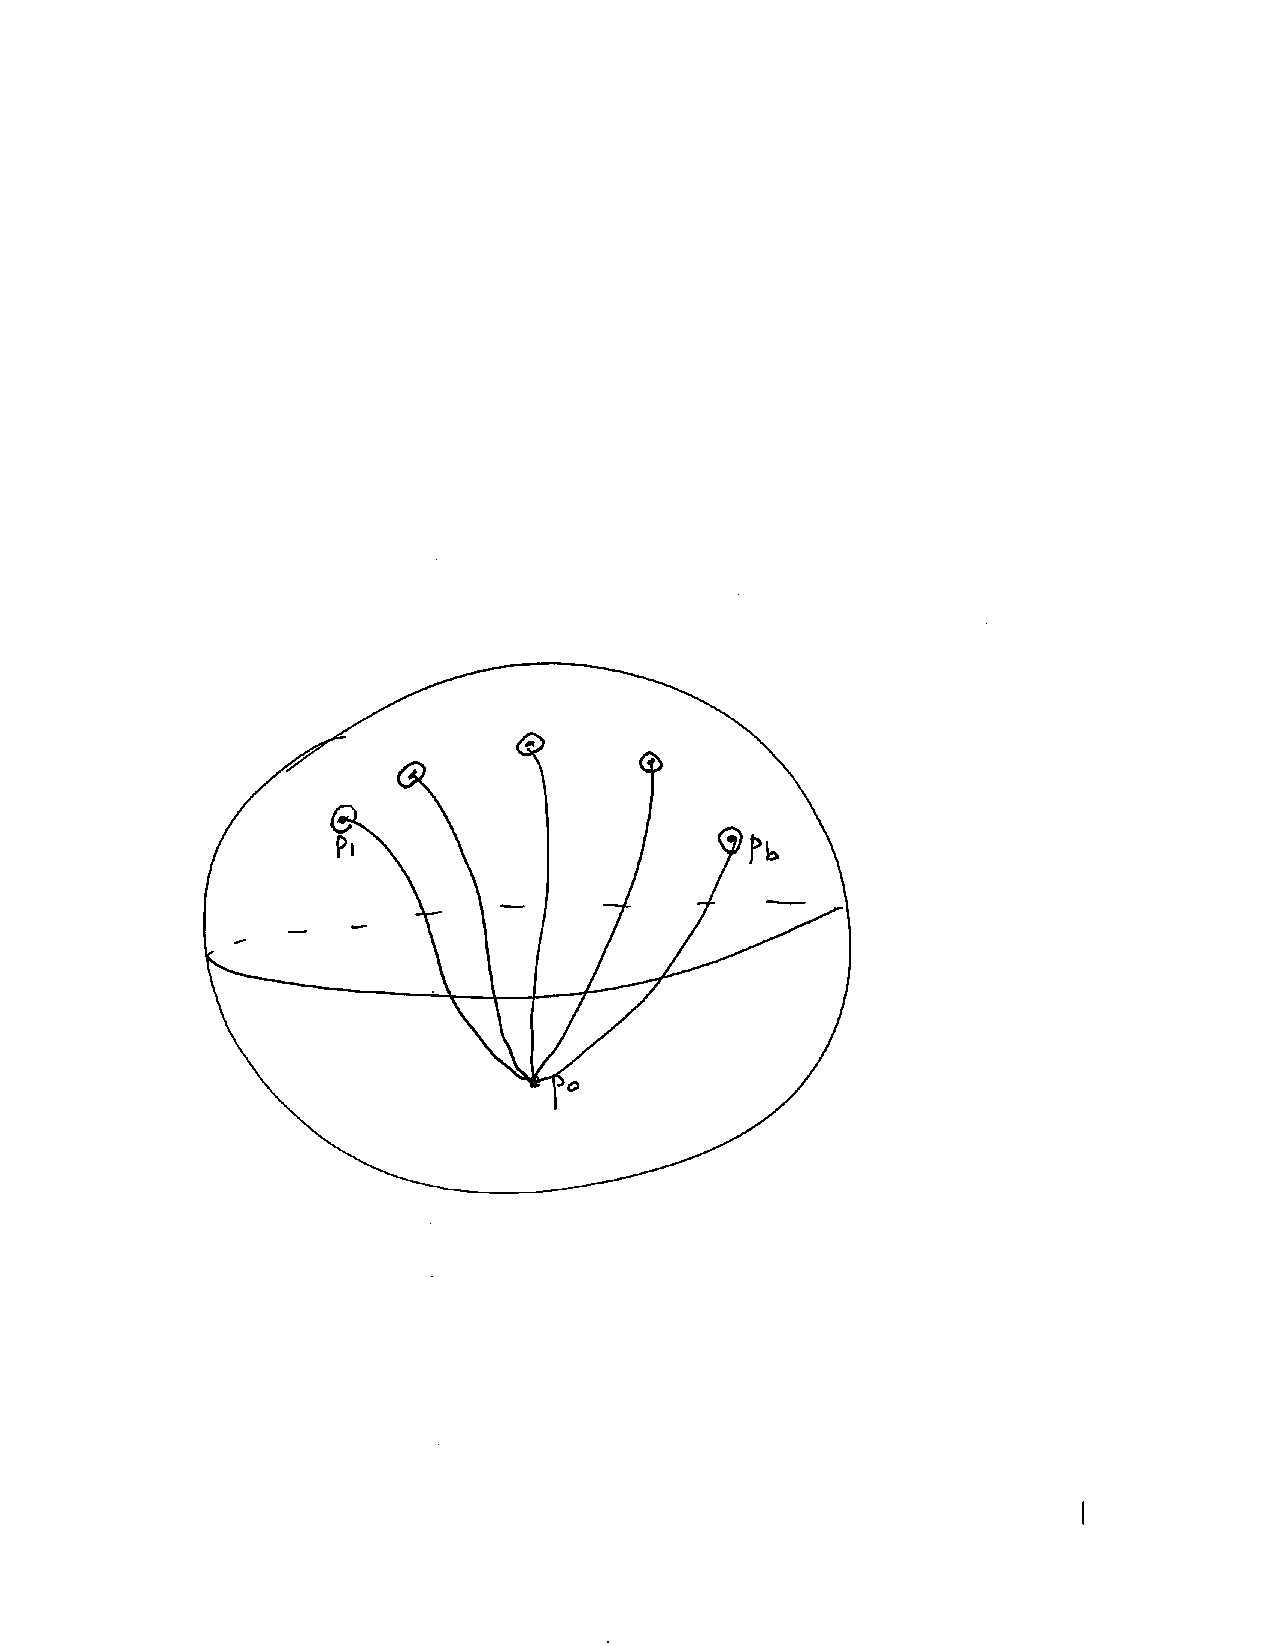
\includepdf{pic4.2}
   
Now, the hypothesis that the cover $\pi : C \to B$ is simply branched amounts to the assertion that $\tau_i$ is a transposition for each $i$. The hypothesis that $V$ is connected says that the subgroup $\langle \tau_1, \dots, \tau_b \rangle \subset S_d$ is transitive. Finally, note that if we were to relabel the sheets $\Sigma_\alpha$ according to some permutation $\sigma$, the effect would be to conjugate each $\tau_i$ by $\sigma$. 

%In sum, then, we conclude that the set of connected, simply branched covers $C \to \PP^1$ of degree $d$ branched over the points $p_1,\dots,p_b$ are in bijection with the set
%$$
%\left\{ (\tau_1,\dots,\tau_b) \mid \tau_i \text{ is a transposition }; \prod \tau_i = id, \text{ and } \langle \tau_1, \dots, \tau_b \rangle \subset S_d \text{ is transitive } \right\}
%$$
%modulo the action of $S_d$ by simultaneous conjugation.
%   
%%   Now consider a small loop around the point $q_i \in \PP^1$, starting and ending a point in $V$. Since the map $\pi : \pi^{-1}(\PP^1 \setminus \Delta) \to \PP^1 \setminus \Delta$ is a covering space, for each $\alpha = 1, \dots, d$ there will be a unique lifting of the loop to an arc in $C$ starting at a point in $V_\alpha$. Suppose now that the endpoint of this lifted arc lies in $V_{\sigma_i(\alpha)}$; in this way, we define a permutation $\sigma_i$ of the set $\{1,\dots,d\}$. Note that by the hypothesis that $\pi$ is simply branched, each $\sigma_i$ is a transposition.
%   
%   There are several things to observe here. The first is that \emph{the data of the collection of transpositions $\sigma_1, \dots, \sigma_b$ determines $C$ as a topological space, and hence as a compact Riemann surface}. Secondly, we observe that the transpositions $\sigma_i$ satisfy two basic conditions: the product $\sigma_1\cdot \dots \cdot \sigma_b$ in the symmetric group $S_d$ is the identity; and the $\sigma_i$ together generate a transitive subgroup of $S_d$. Finally, we note that we could have labelled the sheets $V_1, \dots,V_d$ differently; if we relabel according to a permutation $\tau \in S_d$, the effect will be to conjugate each of the $\sigma_i$ simultaneously by $\tau$.
   
   In sum, then, we have the basic result:
   
   \begin{lemma}
   Let $p_1,\dots, p_b \in \PP^1$ be any $b$ given points. There is a natural bijection between 
   \begin{enumerate}
   \item the set of  simply branched covers $\pi : C \to \PP^1$ of degree $d$, branched over the points $p_i$, up to isomorphism over $\PP^1$ 
%   (that is, we say $\pi : C \to \PP^1$ is equivalent to $\pi' : C' \to \PP^1$ if there exists an isomorphism $\phi : C \to C'$ commuting with $\pi$ and $\pi'$)
   ; and 
   \item the set of $b$-tuples of transpositions $\tau_1, \dots, \tau_b \in S_d$ such that $\prod \tau_i = id$ and such that $\tau_1, \dots, \tau_b$ generate a transitive subgroup of $S_d$, modulo simultaneous conjugation by $S_d$.
   \end{enumerate}
   \end{lemma}

Observe that in the simplest case $d=2$, there is only one transposition in $S_2$, so this says that there is a unique double cover of $\PP^1$ with given branch points $p_1,\dots,p_b$ (it also says that $b$ is even!). This completes the proof of Theorem~\ref{hyperelliptic existence}.

\end{proof}

For a less trivial example, let's count the number of trigonal curves $C \to \PP^1$ with given branch points. This is still relatively simple, given the observation that every odd permutation $\tau \in S_3$ is necessarily a transposition. In other words, if $b$ is even and we specify arbitrary transpositions $\tau_1,\dots,\tau_{b-1} \in S_3$, the product is necessarily a transposition; thus the number of $b$-tuples of transpositions $\tau_1,\dots,\tau_{b} \in S_3$ with $\prod \tau_i = id$ is simply $3^{b-1}$. The requirement that the group generated by the $\tau_i$ is transitive eliminated just the three cases where all the $\tau_i$ are equal; and the group $S_3$ acts on the set of connected covers without stabilizers, so that every cover corresponds to exactly 6 collections $\tau_1,\dots,\tau_b$. In sum, then, we see that \emph{the number of simply branched three-sheeted covers of $\PP^1$ with specified branch points $q_1,\dots,q_b \in \PP^1$ is}
$$
\frac{3^{b-1} - 3}{6}
$$


%
%First, a punctured 2-disk has fundamental group $\ZZ$ and the unique $n$-sheeted covering is again a punctured
%disk; regarding these disks as neighborhoods of the origin in $\CC^2$, the covering map
%can be taken to be $x \mapsto x^n$. This map can of course be extended (by the same formula) to a map
%analytic also at the origin, with ramification index (by definition) $n-1$.
%
%Now suppose that $\Gamma = \{p_1, \dots, p_{d}\}$ is the desired branch divisor.
%Globally, if $\gamma_i$ is a small loop around $p_i$ then the abelianization of the fundamental group $\pi$ of the $d$-times punctured sphere
%$$
%S' := \PP^1\setminus \Gamma
%$$
%is its
%first homology group, 
%$$
%H := H_1(S', \ZZ) = \frac{\oplus \ZZ\cdot \gamma_i}{\ZZ\cdot\sum_i [\gamma_i]}
%$$
%\fix{Insert ``lollipop picture''}. Since $\ZZ/2$ is abelian, a degree 2 unramified covering of $S'$ corresponds to a map $H\to \ZZ/2$, and this map must send $2\gamma_i$ to 0 for $i=1\dots d$.  There is such a map 
%if and only if $d$ is even, and in this case the map is unique. 
%
%Summarizing: there is, a unique degree $2$ topological covering  $C'\to \PP^1\setminus \Gamma$
%by a  surface $C'$ that extends to a ramified covering of $\rho: C\to\PP^1$, simply ramified over the points of
%$\Gamma$, as long as the number of ramification points  is even. 
%
%A triangulation of $\PP^1$ with 
%$V$ vertices including the points of $\Gamma$, $E$ edges, and $F$ triangles must have 
%$$
%V-E+F = \chi_{\rm top}(S^2) = 2.
%$$
% It lifts to a triangulation of $C$ with $2V-d$ vertices, $2E$ edges, and $2F$ faces, so 
%$$
% \chi_{\rm top}(C) = 2V-d-2E+2F = 4-d,
%$$
%so if $d = 2g+2$ then $\chi_{\rm top}(C) = 2-2g$, so $C$ is  a surface of genus $g$.
%
%Though given as a topological surface, the map $\rho$ is a local homeomorphism at every point not in the preimage of $\Gamma$, so $C$ inherits a unique complex structure from the requirement that $\rho$ be holomorphic; thus $C$ is actually a smooth algebraic curve of genus $g$. 
%%\fix{we had better say topological and algebraic genus are the same in the intro.}

As we indicated, there are natural extensions of this basic theory to covers with arbitrary branching, and to covers of curves of any genus. For the first, suppose that instead of specifying ``simply branched"---meaning that the fiber over any branch point consists of $d-2$ simple points and one double point---we specified that the fiber over a given branch point $q_i$ consisted of $m_1$ simple points, $m_2$ double points, $m_3$ triple points and so on. This amounts to specifying a conjugacy class in $S_d$, and instead of associating to $q_i$ a transposition, we want to specify an element of this conjugacy class. Again, the permutations $\sigma_i$ have to have product the identity, and to generate a transitive subgroup of $S_d$; and again, they are determined up to simultaneous conjugation by an element of $S_d$.

\begin{exercise}
Find the number of 3-sheeted covers $C \to \PP^1$ of genus $g$ with simple branching except for one point of total ramification.
\end{exercise}

Similarly, we can similarly enumerate cover of curves $B$ of positive genus by a modification of the construction above. Again, we choose a base point $p \in B$; we can then draw $2g$ loops $\alpha_1,\dots,\alpha_{g},\beta_1, \dots, \beta_g$ based at $p$ and disjoint except for $p$; so that the complement $B \setminus \cup \alpha_i$ is a disc with boundary $\alpha_1, \beta_1, \alpha_1^{-1}, \beta_1^{-1}, \dots, \alpha_g, \beta_g, \alpha_g^{-1}, \beta_g^{-1}$. We then draw arcs $\gamma_i$ joining $p$ to each of the branch points $q_i$. We can then associate to a cover a collection of permutations $\sigma_1, \dots, \sigma_b, \mu_1,\dots,\mu_g, \nu_1,\dots,\nu_g$ (with $\sigma_i$ a transposition, if we are assuming simple branching, or of specified conjugacy class in general, and the $\mu_i$ and $\nu_i$ arbitrary). These determine the cover, and have to satisfy the relation
$$
\prod_{i=1}^b \sigma_i = \prod_{\alpha=1}^g \; [\mu_\alpha, \nu_\alpha]
$$
and of course generate a transitive subgroup of $S_d$

\begin{exercise}
Let $B$ be a given curve of genus $h$. How many unramified double covers of $B$ are there? 
\end{exercise}


\begin{exercise} Let $E$ be a curve of genus 1, and $q_1,\dots,q_b \in E$. How many double covers $C \to E$ are there branched over the $q_i$?
\end{exercise}


\begin{exercise} Let $E$ be a curve of genus 1, and $q, q' \in E$. How many triple covers $C \to E$ are there simply branched over $q$ and $q'$?
\end{exercise}


In general, the numbers of branched covers of a given curve with given branching are called \emph{Hurwitz numbers}; they are of interest to physicists, for reasons we can't fathom.



\section{Curves of genus 2}

%Canonical map to $\PP^1$. Embedding in $\PP^3$ as $(2,3)$ on a quadric, via any degree 5 line bundle. Ideal is 1 quadric, 2 cubics.
%Plane model of degree 4 with node or cusp.

Since  curves of genus 2 are hyperelliptic, everything we said above applies to them; in particular, the canonical map $\phi_K : C \to \PP^1$ on a curve of genus 2 is simply the expression of $C$ as a double cover of $\PP^1$. In this section, we'll consider other maps from $C$ to projective space, starting with maps $C \to \PP^1$.

\subsection{Maps of $C$ to $\PP^1$}\label{genus 2 pencil}

Of course, $C$ may be expressed as a degree 2 cover of $\PP^1$ by taking the map associated to the canonical series $|K_C|$. But what about other degrees? For example, can we express $C$ as a three-sheeted cover of $\PP^1$?

The answer is ``yes," and in fact we can do so in many ways. First start with a line bundle $L$ of degree 3 on $C$. Since $3 > 2g-2$, Riemann-Roch tells us immediately that $h^0(L) = 2$, and we see that there are two possibilities:

\begin{enumerate}
\item First, if the linear series $|L|$ has a base point $p \in C$, then $h^0(L(-p)) = 2$, and hence $L$ must be of the form $L = K_C(p)$. Conversely, if $L = K_C(p)$, then $h^0(L(-p)) = h^0(L)$, which is to say $p$ is a base point of $|L|$.
\item On the other hand, if $L$ is not of the form $L = K_C(p)$, then $|L|$ does not have a base point, and so defines a degree 3 map $\phi_L : C \to \PP^1$.
\end{enumerate}

Do both possibilities occur? Certainly the first does; there's a one-parameter family of line bundles of the form $K_C(p)$. But we know that the variety $\Pic^3(C)$ is 2-dimensional, so we see that the general line bundle of degree 3 does  give an expression of $C$ as a 3-sheeted cover of $\PP^1$; in fact there exists a 2-parameter family of such maps.

\subsection{Maps of $C$ to $\PP^2$} Let's move on to consider maps of our curve $C$ of genus 2 to the plane. By Riemann-Roch, a line bundle $L$ of degree 4 on $C$ will have $h^0(L) = 3$; and since $h^0(L(-p)) = 2$ for any point $p \in C$ (again by Riemann-Roch), we see that the linear series $|L|$ will give a regular map $\phi_L : C \to \PP^2$. We ask now about the geometry of this map.

This again depends on the choice of $L$. This time there are three possibilities:

\begin{enumerate}
\item First, suppose $L = K_C^2$ is simply the square of the canonical line bundle on $C$. We have then a map
$$
\Sym^2 H^0(K_C) \to H^0(L);
$$
since both sides are 3-dimensional vector spaces and the map is injective, we have equality here; in other words, every divisor $D \sim K_C^2$ is the sum of two divisors $D_1, D_2 \in |K_C|$ in the canonical series. To express this in terms of the map $\phi_L$, it says simply that that map $\phi_L$ is the composition of the canonical map $\phi_K : C \to \PP^1$ with the Veronese embedding $\nu_2 : \PP^1 \to \PP^2$ of $\PP^1$ as a conic curve in the plane. In other words, the map $\phi_L$ is generically 2-to-1 onto a conic in the plane.

\item Suppose now that $L$ is not equal to $K_C^2$; equivalently, $M = L \otimes K_C^{-1}$ is a line bundle of degree 2 other than the canonical bundle. We have then $h^0(M) = 1$, so that $M$ is the line bundle $\cO_C(p+q)$ associated to a pair of points $p, q \in C$; in other words, $L = K_C(p+q)$ for a unique pair of points $p, q \in C$.

Let's consider next the general case $p \neq q$. In this case, every section of $L$ vanishing at $p$ vanishes at $q$ and vice versa, so that $\phi_L(p) = \phi_L(q)$. At the same time, for any effective divisor $D = r+s$ of degree 2 on $C$  other than $p+q$, we have $h^0(L(-D)) = 1$, so apart from the fact that $\phi_L(p) = \phi_L(q)$, the map $\phi_L$ is an embedding. We'll see in Exercise~\ref{} below that in fact the point $\phi_L(p) = \phi_L(q)$ is a node of the image curve $\phi_L(C)$; so to summarize: in this case ($L = K_C(p+q)$, with $p \neq q$ and $p+q \neq K_C$), the map $\phi_L : C \to \PP^2$ is a birational embedding of $C$ as a quartic plane curve with one node, the node being the common image of $p$ and $q$.

\item Finally, the remaining case is where $L = K_C(2p)$, where $p \in C$ is any point such that $2p \not\sim K_C$. This behaves much like the preceding case, but here the map $\phi_L$ is one-to-one with vanishing differential at $p$, and the image curve $\phi_L(C)$ has correspondingly a cusp at the point $\phi_L(p)$.
\end{enumerate}

To summarize: the map $\phi_L : C \to \PP^2$ associated to a line bundle $L$ of degree 4 on $C$ is either
\begin{enumerate}
\item Two-to-one onto a plane conic curve, if $L = K_C^2$;
\item Birational onto a plane quartic curve with a cusp, if $L = K_C(2p)$ with $2p \not\sim K_C$; and
\item Birational onto a plane quartic curve with a node, if $L = K_C(p+q)$ with $p \neq q$ and $p+q \not\sim K_C$.
\end{enumerate}

Note that the last case is the ``general" one, meaning it holds for $L$ in an open subset of $\Pic^4(C)$; the second case holds for a one-dimensional locus in $\Pic^4(C)$, and the first case holds for just one point in $\Pic^4(C)$.

\begin{exercise}
Let $L \in \Pic^4(C)$ be a line bundle of the form $L = K_C(p+q)$ with $p \neq q$ and $p+q \not\sim K_C$. Show that
\begin{enumerate}
\item $h^0(L(-2p)) = h^0(L(-2q)) = 1$, and
\item $h^0(L(-2p-2q)) = 0$.
\end{enumerate}
Deduce from this that the map $\phi_L$ is an immersion, and that the tangent lines to the two branches of $\phi_L(C)$ at the point $\phi_L(p) = \phi_L(q)$ are distinct, meaning the point $\phi_L(p) = \phi_L(q)$ is a node of $\phi_L(C)$.
\end{exercise}

%\subsubsection{Representations as double covers of $\PP^1$}
%
%As with curves of genus 1, there are no nontrivial linear series of degree 0 or 1 on a curve of genus 2; the first positive-dimensional linear series occurs in degree 2. Unlike the case of genus 1, however, this series is unique: by Riemann-Roch, if $D$ is any divisor of degree 2 on a curve $C$ of genus 2, we have
%$$
%h^0(D) = 1 + h^1(D) = 1 + h^0(K-D);
%$$
%since $K-D$ has degree 0, this says that $h^0(D) > 1$ if and only if $D=K$, in which case $|D| = |K|$ is the canonical $g^1_2$ on $C$.
%
%The canonical series gives a map $\phi_K : C \to \PP^1$ expressing $C$ as a double cover of $\PP^1$; as in the case of genus 1, this means we can realize $C$ as the smooth projective compactification of the affine curve given by
%$$
%y^2 = x(x-1)(x - \alpha)(x - \beta)(x - \gamma)
%$$
%for some triple $\alpha,\beta,\gamma \in \CC$ distinct from each other and from 0 and 1. This representation shows us that the moduli space $M_2$ is the space of 6-tuples of distinct points in $\PP^1$ modulo the action of $PGL_2$. This tells us immediately that $M_2$ is irreducible of dimension 3; with a fair amount of additional work, we can also use this to describe the coordinate ring of $M_2$ (\ref{**}).

\subsection{Embeddings in $\PP^3$}

So far we have not found any embeddings of $C$ in projective space; but that's about to change: if $L \in \Pic^5(C)$ is any line bundle of degree 5, by Corollary~\ref{degree 2g+1 embedding}, it is very ample and gives an embedding of $C$ in $\PP^3$.
Write $\phi_L : C \to \PP^3$ for the map given by the complete linear system $|L|$. Since $\phi_L$ is an embedding, we'll also denote the image $\phi_L(C) \subset \PP^3$ by $C$ and write $\cO_C(1)$ for $L$.

What degree surfaces in $\PP^3$ contain the curve $C$? We start with degree 2, where we consider the restriction map
$$
H^0(\cO_{\PP^3}(2)) \to H^0(\cO_C(2)) = H^0(L^2).
$$
The space on the left has dimension 10; by Riemann-Roch we have $h^0(L^2) = 2\cdot5 - 2 + 1 = 9$. It follows that $C$ must lie on a quadric surface $Q$; and by Bezout's  theorem  $Q$ is unique (since $C$ can't lie on a union of planes, any quadric containing $C$ must be irreducible; if there were more than one such, Bezout would imply that $\deg(C) \leq 4$).

We might ask at this point: is $Q$ smooth or a quadric cone? The answer depends on the choice of line bundle $L$. 

\begin{proposition}\label{genus 2 embedding}
Let $C \subset \PP^3$ be a smooth curve of degree 5 and genus 2 and $Q \subset \PP^3$ the unique quadric containing $C$. If $L = \cO_C(1) \in \pic^5(C)$, then $Q$ is singular if and only if we have
$$
\cO_C(1) \cong K^2(p)
$$
for some point $p \in C$; in this case, the point $p$ is the vertex of $Q$.
\end{proposition}

Note that the variety $\pic^5(C)$ has dimension 2, while the bundles of the form $K^2(p)$ form a one-dimensional subfamily. Thus in general $Q$ will be smooth, and will become singular in codimension one, as we might expect.

\begin{proof}
First, suppose that the line bundle $L \cong K^2(p)$ for some $p \in C$. Then $L(-p) \cong K^2$, so that the map $\pi : C \to \PP^2$ given by projection from $p$ is the map $\phi_{K^2} : C \to \PP^2$ given by the square of the canonical bundle. As we've seen, the map $\phi_{K^2}$ is two-to-one onto a conic curve $E \subset \PP^2$, so that the curve $C$ lies on the cone $Q$ over $E$ with vertex $p$, and this is the unique quadric surface containing $C$.

Next, let's consider the case where $L$ is not of the form $K^2(p)$. Set $M = LK^{-1}$, so that we can write
$$
L = K \otimes M,
$$
where by hypothesis $M$ is not of the form $K(p)$. As we saw in Section~\ref{genus 2 pencil}, this means that the pencil $|M|$ gives a degree 3 map $C \to \PP^1$.

This gives us a way of factoring the map $\phi_L : C \to \PP^3$: we have maps $\phi_K : C \to \PP^1$ of degree 2 and $\phi_M : C \to \PP^1$ of degree 3, and we can compose their product with the Segre embedding $\sigma : \PP^1 \times \PP^1 \to \PP^3$:
\begin{diagram}
& & \PP^1 & & & &\\
& \ruTo^{\phi_K} & & \luTo & & & \\
C & & \rTo^{\phi_K \times \phi_M} & & \PP^1 \times \PP^1 & \rTo^\sigma & \PP^3 \\
& \rdTo^{\phi_M} & & \ldTo & & & \\
& & \PP^1 & & & & \\
\end{diagram}

This gives us a description of the map $\phi_L$ that shows us immediately that \emph{$C$ is a curve of type $(2,3)$ on a smooth quadric $Q \subset \PP^3$}, completing the proof of Proposition~\ref{genus 2 embedding}.


\end{proof}

Whether the quadric $Q$ is smooth or not, we can describe a minimal set of generators of the homogeneous ideal $I(C) \subset \CC[x_0, x_1, x_2, x_3]$ similarly. First, we look at the restriction map
$$
H^0(\cO_{\PP^3}(3)) \to H^0(\cO_C(3));
$$
since the dimensions of these spaces are 20 and $15-2+1 = 14$ respectively, we see that  vector space of cubics vanishing on $C$ has dimension at least 6. Four of these are already accounted for: we can take the defining equation of $Q$ and multiply it by any of the linear forms on $\PP^3$; we conclude, accordingly, that \emph{there are at least two cubics vanishing on $C$ linearly independent modulo those vanishing on $Q$}.

In fact, we can prove the existence of these cubics geometrically, and show that there are no more than 2 linearly independent modulo the ideal of $Q$. Suppose first that $Q$ is smooth, so that $C$ is a curve of type $(2,3)$ on $Q$. In that case, if $L \subset Q$ is any line of the first ruling, the sum $C+L$ is the complete intersection of $Q$ with a cubic $S_L$, unique modulo the ideal of $Q$; conversely, if $S$ is any cubic containing $C$ but not containing $S$, the intersection $S \cap Q$ will be the union of $C$ and a line $L$ of the first ruling; thus, mod $I(Q)$, $S = S_L$. A similar argument applies in case $Q$ is a cone, and $L$ is any line of the (unique) ruling of $Q$.

\begin{exercise}
Show that for any pair of lines $L, L'$ of the appropriate ruling of $Q$, the three polynomials $Q$, $S_L$ and $S_{L'}$ generate the homogeneous ideal $I(C)$. Find relations among them. Write out the minimal resolution of $I(C)$.
\end{exercise}

%
%\subsubsection{Projective normality III}
%
%\begin{theorem}
% Let $C$ be a smooth (is reduced, irreducible enough?) curve of arithmetic genus $g$, and let $\cL$ be a line bundle on $C$ of degree $\geq 2g+1$. The image of 
% $C$ under the complete linear series $|\cL|$ is projectively normal ( when $C$ is singular, aritmetically Cohen-Macaulay).
%\end{theorem}
%
%\begin{proof}
% The line bundle $\cL$ is very ample by \ref{?}. Thus it suffices We must show that the multiplication map $H^0(\sL)\otimes H^0(\cL^{m}) \to H^0(\cL^{m+1})$ is surjective for all $m\geq 1$.
% For $m=1$ do it by number of quadrics, uniform position. For m>1 the bpf pencil trick.
%\end{proof}

\subsection{The dimension of $M_2$ via maps to projective space}

We remark here that each of the maps we've described from a curve $C$ of genus 2 to projective space gives us a way of finding the dimension of the moduli space $M_2$ of curves of genus 2.

To start, we know that every curve $C$ of genus 2 is uniquely expressible as a double cover of $\PP^1$ branched at six points, modulo the group $PGL_2$ of automorphisms of $\PP^1$. The space of such double covers has dimension 6, and $\dim(PGL_2) = 3$, so we may conclude that $\dim(M_2) = 6-3 = 3$.

Similarly, we've seen that a curve $C$ of genus 2 is expressible as a 3-sheeted cover of $\PP^1$ (with eight branch points) in a 2-dimensional family of ways. Such a triple cover is determined up to a finite number of choices by its branch divisor, so the space of such triple covers has dimension 8; modulo $PGL_2$ it has dimension 5, and since every curve is expressible as a triple cover in a two-dimensional family of ways, we arrive again at $\dim M_2 = 5-2 = 3$.

We've also seen that $C$ can be realized as (the normalization of) a plane quartic curve with a node in a 2-dimensional family of ways. The space of plane quartics has dimension 14; the family of those with a node has codimension one (\ref{PlaneCurvesChapter}) and hence dimension 13. Since  the automorphism group $PGL_3$ of $\PP^2$ has dimension 8, we see that the family of nodal plane quartics modulo $PGL_3$ has dimension 5, and since every curve of genus 2 corresponds to a 2-parameter family of such curves, we have $\dim M_2 = 5-2=3$.

Finally, a curve of genus 2 may be realized as a quintic curve in $\PP^3$ in a two-parameter family of ways. To count the dimension of the family of such curves, note that each one lies on a unique quadric $Q$, and is of type $(2,3)$ on $Q$. Thus to specify such a curve we have to specify $Q$ (9 parameters) and then a bihomogeneous polynomial of bidgree $(2,3)$ on $Q \cong \PP^1 \times \PP^1$ up to scalars; these have $3\cdot 4 - 1 = 11$ parameters. Altogether, then, there is a 20-dimensional family of such curves; modulo the automorphism group $PGL_4$ of $\PP^3$, this is a 5-dimensional family. Again, every abstract curve $C$ of genus 2 corresponds to a 2-parameter family of these curves modulo $PGL_4$, so once more we have $\dim M_2 = 5 - 2 = 3$.

\section{Curves of genus 3}

If $C$ be a smooth projective curve of genus 3. The is an immediate bifurcation into two cases, hyperelliptic and non-hyperelliptic curves; we will discuss hyperelliptic curves of any genus in Section~\ref{**}, and so for the following we'll assume $C$ is nonhyperellitic. By our general theorem~\ref{**}, this means that the canonical map $\phi_K : C \to \PP^2$ embeds $C$ as a smooth plane quartic curve; and conversely, by adjunction any smooth plane of degree 4 has genus 3 and is canonical (that is, $\cO_C(1) \cong K_C$). \fix{maybe a reference to the plane curve chapter
for differentials etc?}

Note that this gives us a way to determine the dimension of the moduli space $M_3$ of smooth curves of genus $3$: if $\PP^{14}$ is the space of all plane quartic curves, and $U \subset \PP^{14}$ the open subset corresponding to smooth curves, we have a dominant map $U \to M_3$ whose fibers are isomorphic to the 8-dimensional affine group $PGL_3$. (Actually, the fiber over a point $[C] \in M_3$ is isomorphic to the quotient of $PGL_3$ by the automorphism group of $C$; but since $Aut(C)$ is finite this is still 8-dimensional.) We conclude, therefore, that
$$
\dim M_3 = 14 - 8 = 6.
$$

%\fix{the following remark seems a little silly, and anyway after saying plane quartic, we DO describe some other models, though with little enthusiasm}
%
%For a non-hyperelliptic curve of genus 3 virtually all the aspects of the geometry of $C$ are best seen in the canonical model.  By contrast, for curves $C$ of other genera, different representations of $C$---as a branched cover of $\PP^1$, as the normalization of a plane curve $C_0 \subset \PP^2$, as embedded in $\PP^3$ and higher-dimensional projective spaces---display different aspects of the geometry of the curve. 

What about other linear series on $C$, and the corresponding models of $C$? To start with, by hypothesis $C$ has no $g^1_2$s; that is, it is not expressible as a 2-sheeted cover of $\PP^1$. On the other hand, it is expressible as a 3-sheeted cover: if $L \in \pic^3(C)$ is a line bundle of degree 3, by Riemann-Roch we have
$$
h^0(L) = 
\begin{cases}
2, &\text{if $L \cong K-p$ for some point $p \in C$; and} \\
1 &\text{otherwise.}
\end{cases}
$$
There is thus a 1-dimensional family of representations of $C$ as a 3-sheeted cover of $\PP^1$. In fact, these are plainly visible from the canonical model: the degree 3 map $\phi_{K-p} : C \to \PP^1$ is just the composition of the canonical embedding $\phi_K : C \to \PP^2$ with the projection from the point $p$. 

There are of course other representations of $C$ as the normalization of a plane curve. By Riemann-Roch, $C$ will have no $g^2_3$s and the canonical series is the only $g^2_4$, but there are plenty of models as plane quintic curves: by Proposition~\ref{**}, if $L$ is any line bundle of degree 5, the linear series $|L|$ will be a base-point-free $g^2_5$ as long as $L$ is not of the form $K+p$, so that $\phi_L$ maps $C$ birationally onto a plane quintic curve $C_0 \subset \PP^2$. But these can also be described geometrically in terms of the canonical model: any such line bundle $L$ is of the form $2K-p-q-r$ for some trio of  points $p, q, r \in C$ that are not colinear in the canonical model, and we see correspondingly that $C_0$ is obtained from the canonical model of $C$ by applying a Cremona transform with respect to the points $p, q$ and $r$. 

We can also embed $C$ in $\PP^3$ as a smooth sextic curve by Proposition~\ref{**}; in fact, a line bundle $L \in \pic^6(C)$ of degree 6 will be very ample if and only if it is not of the form $K+p+q$ for any $p, q \in C$. One cheerful fact in this connection is that these curves are determinantal:

\begin{exercise}
Let $C \subset \PP^3$ be a smooth non-hyperelliptic curve of degree 3 and genus 6. Show that there exists a $3 \times 4$ matrix $M$ of linear forms on $\PP^3$ such that 
$$
C = \{ p \in \PP^3 \mid \rank(M(p)) \leq 2 \}.
$$
\end{exercise}

\input footer.tex


